\label{sec:kuramoto}

\subsection{Definition}
The problem of having a naive viewpoint on the subject of synchronization is that one may believe that every different coupling situation would require its own treatment. This may stem from the fact that one may be focusing too much on the differences rather then the similarities which are found in all synchronous systems.  In this project we want to use the model of oscilators that was first introduced by Kuramoto in ~\cite{book:kura}. The most common form is given by the following system of ODEs:

\[
\dot{\theta_i} = \omega_i + \sum_{j = 0}^{N}{A_{i, j}\sin({\theta_j - \theta_i}}) + B_i \sin(\Omega(t) - \theta_i)\]

\ednote{What does each coeeficient in this form mean?}
Here 
\begin{itemize}
	\item[${\theta_i} = $] The phase of the $i\textsuperscript{th}$ oscillator
	\item[$\omega_i = $] The natural frequency of the $i\textsuperscript{th}$ oscillator
	\item[$A_{i, j} = $] The adjacency matrix of the system
	\item[$\Omega(t) = $] An External Driver on the system
	\item[$B_i = $] The vector containing coefficients of the external oscillator. The higher these coefficients, the stronger the influence from the external driver
\end{itemize}
~\\
Each oscillator has its own natural frequency which is held when kept in isolation but when coupled with other oscillators, it changes. This change is periodic and is thus represented by the periodic $\sin$ function. It should be noted that any periodic function can be taken. Sometimes, even a constant function is taken to make the equation simpler.

\subsection{The Adjacency matrix and network topology}

\ednote{Link to the above: Each oscilator can be seen as a node in a network?}

Now we move on to define the mathematical tools being used in this project. The Adjacency matrix is a square matrix that is using to represent a finite graph. The elements of the matrix indicate whether pairs of verticies are adjacent or not, ie if they are adjacent they get assigned a value of -1 else 0. This information can be directly retrieved from the topology network graph as follows-:

\begin{figure}[h!]
\centering
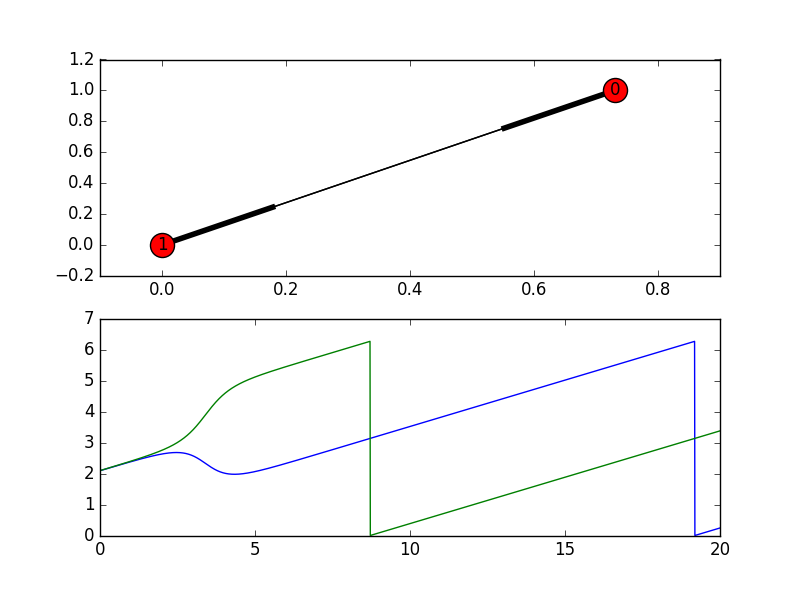
\includegraphics[width=0.8\linewidth]{imgs/examplefigure}
\caption{}
\end{figure}

As we can see, on the top is the topological network containing the vertices of the system and below lies the coupling graphs of the system over time. Over here, we can see that the couples are trying to stay as far away as possible so after the initial unrest there is always a phase difference of 2$\pi$. \ednote{JUST show the graph and the adjacency matrix here. This is ONLY the introduction. }


\subsection{Our implementation}
The following code line illustrates the gist of how we used the NumPy package to compute the $\sin$ of the phase differences and the standard ode solver to numerically estimate the solution.
\begin{lstlisting}
if (self.A[i, j] != 0) and (i != j):
s.append('(%s)*np.sin(theta[%s] - theta[%s])' % (self.A[i, j], j, i))

if self.B[i] != 0:
s.append('(%s)*np.sin((%s)*t - theta[%s])' % (self.B[i], self.OMEGA, i))

sol = odeint(self.to_equation(), y0, t, *args, **kwargs)
\end{lstlisting}
Basically, we just append the calculated values into an array and later solve that using the ODE solver. As an example, I will demonstrate using a random 3x3 graph with no external driver. The adjacency matrix of the graph is-:
\[
\begin{bmatrix}
	\centering
	0 & 1 & 1\\ 
	1 & 0 & 1\\ 
	1 & 1 & 0
\end{bmatrix}
\]
Since its a 3x3 matrix, there will be 3 oscillators. Everything except the diagonals are 1 which means all the oscialltors are connected with each other but not with themselves. Therefore, we get the expected graph-:
\begin{figure}[h!]
	\centering
	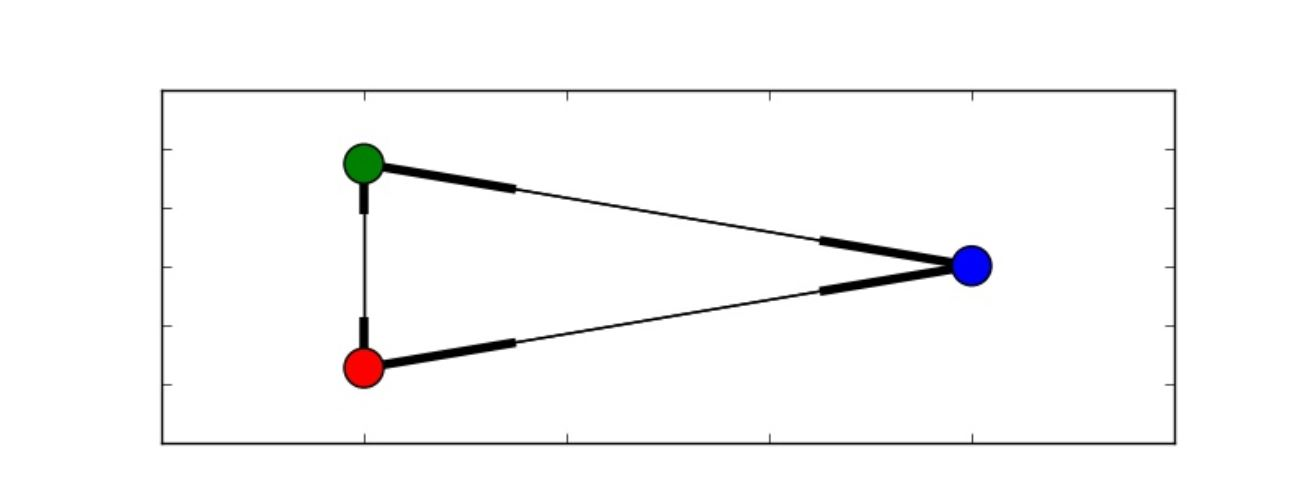
\includegraphics[width=0.8\linewidth]{imgs/examplefigure2}
	\caption{}
\end{figure}


\ednote{Alee: Write about the simulation we have written, i.e. we used Numpy, we have a script that can handle arbritrary parameters and make a simple **positive coefficient** system where you can explain the connection. }
